\usetikzlibrary{calc}


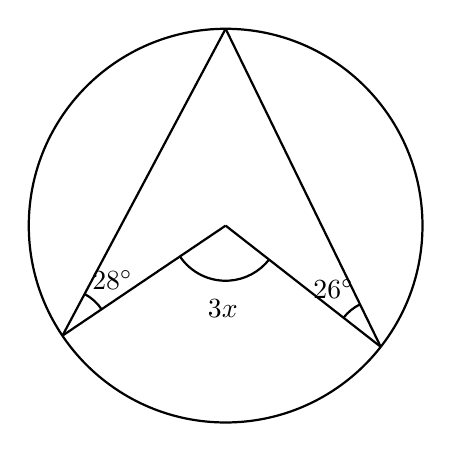
\begin{tikzpicture}[scale=1]

    % Define the center of the circle
    \coordinate (O) at (0,0);

    % Define the points on the circle based on geometric calculations
    % Top vertex (placed symmetrically at the top)
    \coordinate (A) at (90:2.5);
    
    % Bottom left vertex
    % Calculated so the angle between the chord to A and the radius to O is exactly 28 degrees
    \coordinate (B) at (214:2.5);
    
    % Bottom right vertex
    % Calculated so the angle between the chord to A and the radius to O is exactly 26 degrees
    \coordinate (C) at (322:2.5);

    % Draw the circle
    \draw[thick] (O) circle (2.5);

    % Draw the chords connecting the top vertex to the bottom vertices
    \draw[thick] (A) -- (B);
    \draw[thick] (A) -- (C);
    
    % Draw the lines from the bottom vertices to the center
    \draw[thick] (B) -- (O);
    \draw[thick] (C) -- (O);

    % Draw the angle arcs and place the labels exactly as shown in the image

    % 28 degree angle arc at vertex B
    % The radius to O is at 34 degrees, the chord to A is at 62 degrees
    \draw[thick] (B) ++(34:0.6) arc (34:62:0.6);
    \node at ($(B) + (48:0.95)$) {$28^{\circ}$};

    % 26 degree angle arc at vertex C
    % The chord to A is at 116 degrees, the radius to O is at 142 degrees
    \draw[thick] (C) ++(116:0.6) arc (116:142:0.6);
    \node at ($(C) + (129:0.95)$) {$26^{\circ}$};

    % 3x angle arc at the center O
    % The line to B is at 214 degrees, the line to C is at 322 degrees
    \draw[thick] (214:0.7) arc (214:322:0.7);
    \node at (268:1.05) {$3x$};

\end{tikzpicture}